\documentclass[a4paper,12pt]{article}
\usepackage[latin1]{inputenc}     % pour Unix Latin1 aussi..
% \usepackage[applemac]{inputenc} % pour utilisateurs mac
% \usepackage[ansinew]{inputenc}  % pour Windows ANSI (yen a encore qui utilisent ca? :s)
\usepackage{verbatim} 
\usepackage{aeguill}
\usepackage{amsfonts}
\usepackage{xspace}
\usepackage{amsmath}
\usepackage{lscape} % pour avoir une page en paysage
\usepackage{fancybox}
\usepackage{fancyhdr}
\usepackage{textcomp}  % pour les caract�res sp�ciaux (copyleft etc)
\usepackage{marvosym} % caractere electrostatic, laserbeam...
\usepackage{supertabular}% tableaux sur plusieurs pages
\usepackage{ifsym} % caract�res scp�ciaux
\usepackage{longtable}
\usepackage{upgreek}
\usepackage{picins}
\usepackage{lastpage}
\usepackage[english,french]{babel}
%%%%%%%%%%%%% parallel, multicolpar et parcolumns.%%%%%%%%%%%%%%%%%%%%%% pour des documents multicolones bilingue.
\usepackage[pdftex]{graphicx, color}
\usepackage{pdfpages}
\graphicspath{{img/}} % La ou j'ai mes images
\DeclareGraphicsExtensions{.jpg,.png}
\pdfoutput=1
\usepackage[pdftex,
	a4paper,
        bookmarks = true,           % Signets
        bookmarksnumbered = true,   % Signets numerotes
        pdfpagemode = None,         % Signets/vignettes fermes a l'ouverture
        %pdfstartview = FitH,        % La page prend toute la largeur
	pdfstartview = FitV,        % La page prend toute la hauteur
	colorlinks=true,
	citecolor=black,urlcolor=blue,linkcolor=red,
	pdfauthor={K�vin Raymond},
	pdftitle={Stage au CERN},
 	pdfsubject={Rapport de stage},
	pdfkeywords={Xbee, pt100, PIC, GNU,Piklab, SDCC, Linux, CAO, gEDA},
	plainpages=false,
	pdfpagelabels,
	bookmarks,
	breaklinks=true,
   	hyperindex,
	linktocpage=true	% pour colorier seulement le num�ros dans la TOC	
]{hyperref}
%
\pdfcompresslevel=9
%
%
%%% style sans serif pour les url
\urlstyle{sf}

%



%%%% debut macro %%%%
\newenvironment{changemargin}[2]{\begin{list}{}{%
\setlength{\topsep}{0pt}%
\setlength{\leftmargin}{0pt}%
\setlength{\rightmargin}{0pt}%
\setlength{\listparindent}{\parindent}%
\setlength{\itemindent}{\parindent}%
\setlength{\parsep}{0pt plus 1pt}%
\addtolength{\leftmargin}{#1}%
\addtolength{\rightmargin}{#2}%
}\item }{\end{list}}
%%%% fin macro %%%%

%
%
%%%%%%%%% Mise en Forme page de garde %%%%%%%%%%%%%%%%%%%%
%######################## D�finition du titre ######################
\title{
\thispagestyle{empty}
\vspace{-40mm}
   \begin{minipage}[c][150pt][c]{.40\linewidth} %[hauteur][position]{largeur}
		\begin{flushleft}
		\vspace{2mm}
		
\includegraphics[width=3cm]{./img/CERN_logo}
		\vspace{3mm}
		\end{flushleft}
   \end{minipage}\hfill
   \begin{minipage}[c][150pt][c]{.40\linewidth} %[hauteur][position]{largeur}
	{\normalsize 
		\begin{flushright}
		\vspace{3mm}
		\textsc{K�vin Raymond}\\
		Ann�e 2007\\
		\end{flushright}
	}
   \end{minipage}
\vfill
\rule{\linewidth}{0.8mm}\vspace{6mm}\\
    \begin{minipage}[c]{0.70\linewidth} %[hauteur][position]{largeur}
	{\large	
		Utilisation de gEDA, suite libre de CAO\\
		Programmation des PIC sous Linux\\
		Utilisation de la carte Mesure de temp�rature\\
	}
	\end{minipage}\vspace{6mm}
\rule{\linewidth}{0.8mm}\vspace{6mm}\\
\vspace{3mm}
\begin{minipage}[c][150pt][c]{.40\linewidth} %[hauteur][position]{largeur}
	{\normalsize 
		\begin{flushleft}
		\textbf{R�sum�~:}\\
		Article d�stin� � aider � prendre en main la suite de CAO gEDA, Piklab pour programmer les PIC sous linux et quelques notes sur l'utilisation de la carte pour mesurer les temp�ratures.
		\end{flushleft}
	}
   \end{minipage}
\date{} % Je ne veux pas afficher la date
}  %fin du titre



%
%%%%%%%%%%%%%%%% Fin des includes... %%%%%%%%%%%%%

\begin{document}

%%
\maketitle

\newpage

\setcounter{page}{1} %On definit un compteur a 1
\pagenumbering{roman} %permet une num�rotation en chiffre romain

%%
\tableofcontents
\newpage



\setcounter{page}{1} % On r�initialise le coompteur des pages
\pagenumbering{arabic} % On repasse en num�rotation en chiffre Arabe
\pagestyle{fancy}
\section*{Introduction}
\addcontentsline{toc}{section}{Introduction}

Cet article est d�stin� � favoriser la prise en main de gEDA, suite libre de Conception �lectronique Assist� par Ordinateur.
Ce n'est en aucun cas une documentation suffisante, il a pour but de compl�ter les articles r�dig�s par les concepteurs.

Nous verrons �galement de quel mani�re programmer les PIC (microcontr�leurs de chez Microchip) sous Linux en C. 

Finalement nous �tudierons les cartes �lectroniques permettant la mesure d'une temp�rature avec les sondes Pt100.

 
 \newpage
\section{gEDA}
Les logiciels de Conception �lectronique Assist� par Ordinateur (CAO) propri�taires sont une bonne solution pour d�buter rapidement et obtenir simplement des cartes exploitables. 

Mais ne serait-il pas plus souhaitable d'utiliser un outil compl�tement personnalisable avec lequel on n'obtient tr�s rapidement des cartes au rendu professionel~? Ceci est possible gr�ce aux logiciels libres. gEDA en est id�al pour la CAO. C'est un outil en plein d�veloppement mais d'ores et d�j� �volu�. 

De nombreuses librairies sont disponibles et il est tr�s rapide d'en ajouter. Il en existe deux m�canismes. Le premier appel� \og Oldlib \fg\, \og pcblib \fg\ ou \og biblioth�que M4 \fg\ d�pend du langage macro M4. Les empreintes sont g�n�r�es � la vol�e. \` A utiliser pour creer rapidement des familles d'empreintes. Le deuxi�me m�canisme est appel� \og Newlib \fg . Ce sont les empreintes que l'on peut creer graphiquement avec Pcb, ou avec un �diteur de texte (code ASCII). \newline

gEDA pour GPL Electronic Design Automation est une suite Open Source permettant la cr�ation de sch�mas, la simulation et la r�alisation du Printed Circuit Board (PCB). \newline

Cette suite d'outils est principalement compos�e de :
\begin{itemize}
\item[-] \textbf{gschem}, l'�diteur de sch�mas et de symboles,
\item[-] \textbf{gnetlist}, un translateur vers d'autres utilitaires,
\item[-] \textbf{PCB}, un outil de dessins de circuits imprim�s et de cr�ation d'empreintes,
\item[-] \textbf{ngspice}, un clone de spice avec des fonctions �tendues,
\item[-] \textbf{gnucap}, un simulateur original avec compilateur de mod�les,
\item[-] \textbf{geda}, le gestionnaire de projet (non actuel).
\end{itemize}

\vspace{5mm}
Attention � l'utilisation de geda le gestionnaire de projet. Il n'a pas suivi l'�volution des autres programmes, il est donc pr�f�rable de ne pas l'utiliser. Un terminal suffit pour relier les diff�rents outils.\newline

%%

\subsection{installation}
Avant tout il faut l'installer. La derni�re version de gEDA n�cessite python 2.5 ou sup�rieur. Il est possible que gEDA, ainsi que toutes ses d�pendances, soit dans les d�p�ts de votre distribution (voir par exemple avec Synaptic). Mais ce ne sera peut-�tre pas la derni�re version. Pour cette suite en constante �volution il est important d'avoir la derni�re version, pour �viter certains bogues.\newline


Une autre possibilit� est de t�l�charger l'image iso du CD. Elle inclut la derni�re version de tous les programmes. Ainsi que les d�pendances n�cessaires. Voir dans la partie download du site officiel : \url{http://www.geda.seul.org/}\label{sitegEDA}. La solution la plus simple est de monter le cd sur un lecteur virtuel. Tr�s simple sous linux.
\begin{center}
\ovalbox{\$ sudo mount -oloop <image>.iso /mnt} 
\end{center}
\vspace{2mm}

Pour poursuivre l'installation l'aide n�cessaire se trouve sur le CD. En ce qui concerne les tutoriaux, attention � bien lire les derni�res versions.\newline


Une fois l'installation termin�e, il faut avoir le synoptique de la suite logicielle en t�te pour commencer une carte.
\begin{center}
\begin{figure}[h!]
	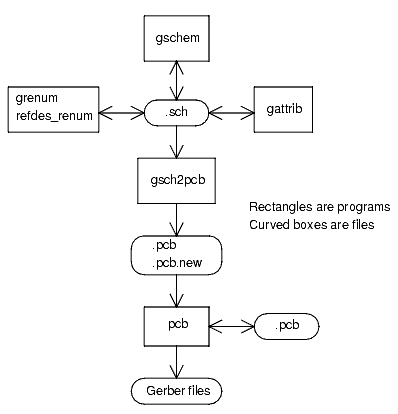
\includegraphics[width=8cm]{./img/gedaSy}
	\caption{Synoptique de la suite gEDA}
\end{figure}
\end{center}
\vspace{2mm} 

Tout commence avec gschem. Une fois le sch�ma r�alis� et v�rifier avec le contr�leur DRC il faut cr�er la netliste. Grenum sert � assigner une r�f�rence � tous les composants. Ce qui peut �tre r�alis� automatiquement avec gschem. De m�me gattrib permet d'assigner des empreintes aux composants. Mais il est plus �vident au d�but de le faire sous gschem. 
gsch2pcb permet de cr�er la netlist et le fichier *.pcb. Pcb permet de placer les composants et de router les connexions g�n�r�es par la netlist. Enfin, les fichiers Gerber sont export�s par Pcb.


%%
\subsection{gschem}
gschem est un logiciel permettant de rapidement cr�er des sch�mas pour peu que nous l'ayons bien en main. Il existe une multitude de raccourcis permettant d'aller plus vite. \newline

Il est conseill� de cr�er un dossier de projet, car de nombreux fichiers seront cr��s. Une fois gschem ouvert (commande \og gschem\fg), vous verrez une interface simple d'utilisation~: seulement quelques ic�nes sont dans la barre des t�ches. Possibilit� d'ajouter des composants, de cr�er des fils de connexion voire des bus de donn�es. Pour tourner les composants ou toute autre t�che utile, il est bien plus rapide de se servir des raccourcis.
gschem �tant en fran�ais, il est tr�s rapide de trouver les fonctions d�sir�es.\newline

En vue de simplifier la g�n�ration de la netlist, veuillez � bien renseigner au minimum trois champs importants pour gschem. 

Double-cliquer sur un composant pour ouvrir ses propri�t�s. En g�n�ral le champ \textbf{device} et  \textbf{refdes} est rempli. Le champ de loin le plus important est \textbf{footprint}, il permet de sp�cifier quelle empreinte prendre pour ce composant. N'importe quel symbole (ou composant) peut appeler n'importe quelle empreinte. Cela permet de cr�er une seule empreinte pour plusieurs composants. Ils seront diff�renci�s sous Pcb par leur identifiant device et refdes. Une fois les composants ajout�s, il est possible de renseigner automatiquement tous les champs refdes par \og Attributs -> Annotation automatique\fg. Les champs slot et numslot permettent de sp�cifier le num�ro de la porte  lorsqu'il y en a plusieurs par bo�tier.\newline

Lors de la cr�ation de symboles il faut sp�cifier le champ \textbf{pintype} pour que le v�rificateur d'erreurs (DRC) puisse v�rifier les erreurs de connexions. Les diff�rentes options pour ce champ sont \og io\fg\ pour une entr�e-sortie, \og pas\fg\ pour une broche passive, \og in\fg\ pour une entr�e, \og out\fg\ pour une sortie et \og pwr\fg\ pour une alimentation.\newline

Une fois que le sch�ma est fini, il faut le v�rifier avec le DRC puis corriger les erreurs. Lancer le code ci-dessous dans un terminal au m�me endroit que votre projet.

\begin{center}
\ovalbox{\$ gnetlist -g drc2 text.sch -o drc\_output.txt} 
\end{center}

le r�sultat de DRC est visible dans le fichier drc\_output.txt. \newline

Personnellement, je trouve plus simple de lire le r�sultat directement dans la console:
\begin{center}
\ovalbox{\$ gnetlist -g drc2 text -o -} 
\end{center}

Si vous rencontrez une erreur du type 

\begin{quote}
Checking slots~\dots\newline
ERROR: Reference U5: Slot out of range (1).\newline
slotnumber~=~1\newline
\end{quote}

Vous avez s�rement une empreinte avec un nom finissant par une minuscule. Ce qui est interpr�t� comme le num�ro d'une porte logique � l'int�rieur d'un composant. S'il ne s'agit pas d'une erreur il est possible de passer outre en sp�cifiant le champ \textbf{numslot} � 0.\newline


La netlist est cr�e en m�me temps que le rapport du DRC, il faut donc maintenant invoquer gsch2pcb pour commencer le routage.
\begin{center}
\ovalbox{\$ gsch2pcb -v text.sch} 
\end{center}
L'option verbose (-v) est facultative, mais permet de suivre les diff�rentes erreurs dues principalement � des empreintes introuvables. La double option verbose (\$~gsch2pcb~-v~-v~text.sch) permet de voir tous les fichiers scann�s pour trouver les diff�rentes empreintes.
Lorsqu'il n'y a plus d'erreurs, il faut passer sur Pcb. Le fichier text.pcb est cr�� par gsch2pcb. Il faut maintenant l'ouvrir avec Pcb.\newline

Je pr�cise que les principales d�marches � suivre sont rappel�es par gsch2pcb � la fin du rapport. Lors d'une premi�re ex�cution on peut lire par exemple:

\begin{quote}
Next step:
\begin{itemize}
\item[1.]  Run pcb on your file test.pcb.
    You will find all your footprints in a bundle ready for you to place
    or disperse with \og Select -> Disperse all elements\fg\ in PCB.

\item[2.] From within PCB, select \og File -> Load netlist file\fg\ and select 
    test.net to load the netlist.

\item[3.] From within PCB, enter
		:ExecuteFile(test.cmd)\newline
\end{itemize}
\end{quote}
 

Lors d'une mise � jour (le fichier test.pcb existe d�j�) d'autres conseils apparaissent :
\begin{quote}
Next steps:
\begin{itemize}
\item[1.] Run pcb on your file test.pcb.
\item[2.] From within PCB, select \og File -> Load layout data to paste buffer\fg\
    and select test.new.pcb to load the new footprints into your existing layout.
\item[3.] From within PCB, select \og File -> Load netlist file\fg\ and select 
    test.net to load the updated netlist.

\item[4.]From within PCB, enter
           :ExecuteFile(test.cmd)\newline
\end{itemize}
\end{quote}


Dans tous les cas la prochaine �tape est Pcb.


%%%%
\subsection{Pcb}
\parpic[r]{
\includegraphics[width=25mm]{./img/pcb}}Je conseille d'ouvrir directement Pcb par un autre terminal puisque le programme retourne un certain nombre d'erreurs (notamment \og unknown action\fg\ pour une commande inconnue) . Proc�der par \ovalbox{\$~pcb~test.pcb} tout en �tant dans le r�pertoire du projet.\newline
Pcb ouvre automatiquement une fen�tre de log qui retourne les diff�rentes actions de l'utilisateur prises en compte par le programme.\newline

Une fois le fichier test.pcb ouvert il faut r�organiser les composants (Select -> Disperse all elements).
Il ne reste plus qu'� importer la netlist (File~->~Load netlist file). Ensuite lancer le fichier test.cmd par l'invite de commande (le raccourci pour cette action est [:]). \ovalbox{ExecuteFile(test.cmd)}. Puis remettre � jour. Action possible par la touche de raccourci [O]. 
Si les fils de connexions (ratsnet) ne sont pas visibles, activer l'option en cliquant sur le bouton \og ratsnet\fg\ (� gauche).\newline

\begin{center}
\shadowbox{
\begin{minipage}{0.7\textwidth}
Pour mettre � jour le PCB si un changement doit appara�tre (modification sous gschem des connexions ou composants par exemple), lancer le DRC pour v�rifier et r�g�n�rer la netlist, ce qui a pour effet de cr�er un fichier test.pcb.new. Ouvrir ce fichier par \og File -> Load layout-data to past buffer \fg. Recharger la netlist, lancer la commande ExecuteFile(test.cmd) et r�actualiser les fils de connexions ([O]). 
\end{minipage}
} \newline
\end{center}



{\Large Pour une prise en main assez rapide de Pcb:\newline}

Dans la barre d'outils verticale (sur la gauche) il est possible de s�lectionner l'affichage des plans, via, pistes etc. Par d�faut il existe plusieurs couches avec une couleur pour chaque signal (alimentation, donn�es~\dots). Il est possible de modifier ces options par \og File -> Preference\fg.

En dessous sont repr�sent�s les outils de dessins. Line pour les pistes, polygon pour les plans de masses par exemples, LOCK pour v�rouiller un composant. Utile par exemple pour les plans ou les gros composants, cela �vite de le s�lectionner alors que l'ont visait une piste. L'outil THRM permet rapidement d'ajouter ou d'enlever des freins thermiques aux pastilles.

Pour d�placer un composant avec ses pistes (ou ratsnet), le clic souris suffit. Parfois il est pr�f�rable de d�placer un composant sans ses connexions. Pour cela il faut le s�lectionner (clic souris) puis le d�placer par un autre clic souris.

Plusieurs actions sont disponibles par [shift]+Clic droit. Notamment supprimer l'ensemble de la s�lection.
La touche [Shift] lors d'un trac� de piste sert � modifier la position de l'angle. Tr�s pratique!

Pour une mesure rapide [CTRL]+[M] r�-affecte l'origine (les mesures sont en haut � droite). Pour avoir la vue de la face de dessous il suffit de presser la touche [TAB]. Alors que [B] permet de passer le composant d'une face � l'autre. 

[U] pour \og Undo\fg\ (annuler) et [Shift]+[R] pour \og Redo\fg\ (restaurer). 

[Q] permet de modifier l'apparence des pastilles (rondes ou carr�es).[D] permet d'afficher rapidement le num�ro des broches et [shift]+[D] en donne l'apper�u. 

[O] qui permet de r�actualiser les connexions est souvent utilis�e de m�me que [F] qui permet de mettre en surbrillance les connexions directes. [S] et [shift]+[S] servent � modifier la taille des pastilles, pistes, etc. 

[V] permet d'avoir une vue globale de la carte. Pour le reste des raccourcis utilis�s, voir dans \og Window -> Key References\fg.\newline

Attention � bien activer l'option \og Settings -> New lines, arcs clear polygon\fg\ si vous devez faire un plan de masse ou autre par la suite. \` A d�faut vous retrouverez toutes vos pistes court-circuit�es par le plan. Attention cela pose probl�me pour les freins thermiques. Citation: \og � consommer avec mod�ration\fg.

Cependant il est toujours possible d'activer l'option � la fin,  un travail assez r�barbatif.
Dans les tutoriaux on peut trouver la commande \og :changejoin(selected)\fg\ pour changer l'option sur toutes les pistes s�lectionn�es, mais cela n'avait aucun effet sur ma version. D�couvert par le \og unknown action\fg\ retourn� dans le terminal. La touche raccourci pour le m�me r�sultat est [shift]+[J]. Il est possible de modifier la clearance des pistes (espace vide entre la piste et le plan) par la touche [K] (et [shift]+[K]).\newline

Lorsque vous avez le programme en main, il est tr�s rapide de router ses cartes puisque le logiciel permet d'un clic de copier des �l�ments dans un tampon (�l�ments pr�c�demment cr��s). On peut donc avoir � port�e de clic des dessins souvent utiles (logo, empreinte de frein thermique, etc.)\newline

{\Large Cr�er des empreintes (Footprint):}\newline 

Partir d'un �l�ment existant est le plus rapide. Il est possible (et tr�s utile, pour v�rification notamment) de cr�er des empreintes directement sur notre PCB. 

Pour ce faire, ouvrir le gestionnaire de librairie par \og Window~->~library\fg. Ajouter le composant le plus ressemblant. Le s�lectionner pour ensuite le copier dans le buffer ([CTRL]+[X]). Maintenant il faut le convertir en \og pi�ce\fg\ : \og Buffer~->~Convert~buffer~to~pieces\fg. Coller cette pi�ce. 

Il est maintenant possible de jouer avec tous ces �lements. Num�roter les broches avec la touche [N]. Une fois toutes les modifications effectu�es, copier la pi�ce dans le buffer puis \og Buffer~->~Convert~buffer~to~elements\fg\ pour enfin l'enregistrer \og Buffer~->~Save~buffer~to~File\fg.

Noter que les pastilles \og carr�es\fg\ sont obtenues par des lignes \og arrondies\fg\ et ensuite modifi�s avec la touche [Q] (une fois converties en �lement).\newline

\textbf{Attention, si le nom des empreintes contient une minuscule comme dernier caract�re, elle sera consid�r�e comme une porte � l'int�rieure d'un autre composant (souvent nomm�e a, b, c~\dots) Elles seront ignor�es. Il faut mettre un chiffre ou une majuscule.}\newline

Pour plus d'informations : \newline
\url{http://ronja.twibright.com/guidelines/footprints.php}, pour une plus grande explication sur la cr�ation d'empreintes graphiques (par Pcb).\newline
\url{http://www.brorson.com/gEDA/land_patterns_20050129.pdf}, un tutoriel pour dessiner ses empreintes � la main, avec un �diteur de texte.\newline




Une fois le PCB termin�, d'un clic on peut exporter la carte en fichier Gerber, png, ps, eps~\dots 



%\section{Conclusion sur gEDA}

Une des plus grandes richesses de gEDA est le traitement des donn�es entre les diff�rents programmes. Tous les fichiers sont en ASCII ce qui les rend tr�s facile � manipuler. Il est donc possible de se cr�er des scripts pour automatiser des t�ches r�barbatives. Habituellement le Perl est utilis� pour cela. Voici les scripts distribu�s par gEDA~:\newline
\begin{itemize}
\item[1.] John Luciani poss�de un large �ventail de scripts disponibles sur son site we (\url{http://www.luciani.org/}). Dans cette collection, des scripts sont inclus pour g�n�rer des empreintes, notamment Footgen.
\item[2.] David Rowe poss�de des scripts pour mettre � jour des �l�ments de m�me qu'ajouter/supprimer des fichiers PCB les uns des autres sur son site web (\url{http://www.rowetel.com/perl4pcb.html}).
\item[3.] Stuart Brorson a �crit un script simple qui g�n�re des empreintes pour deux ponts thermiques passifs en SMD. Un tarball gzipp� est disponible � \url{http://www.brorson.com/gEDA/Smtgen.pl.gz}.\newline
\end{itemize}


Une fois en main, gEDA est � la fois simple et rapide � utiliser. De plus beaucoup de librairies sont disponibles sur \textbf{\url{http://www.gedasymbols.org/}}. Il est �galement possible de demander sur la liste des geda-user si ce composant est disponible. Pour cela voir \url{http://geda.seul.org/mailinglist/index.html}. \newline

Pour la recherche de librairies, suivre les liens pr�c�demment cit�s ou \textbf{\url{http://www.gedasymbols.org/}}. On en apprend �galement beaucoup sur \url{http://www.geda.seul.org/wiki/geda:usage.fr}.\newline

Sur divers sites internet on trouve des tutoriaux pour gEDA, mais en g�n�ral ils ne sont pas � jour. Tout le probl�me est l�. Les plus int�ressants sont les tutoriaux des logiciels et non de la suite. Eux sont � jour. Je pense par exemple au tutorial de Pcb disponible sur \url{http://pcb.sourceforge.net/manual.html}. Pour comprendre un peu mieux la gestion d'un projet sous gEDA il peut �tre utile de lire le tutorial en Fran�ais disponible l�~: \url{http://www.iznogood-factory.org/pub/gEDA/tutorialfr.html}. Il n'est pas bas� sur la derni�re version, car certaines configurations ont chang�es. Sur ce site (\url{http://ofset.sourceforge.net/freeduc/book/book_29.html}) est disponible un exemple rapide de prise en main de Pcb. En lisant plusieurs tutoriaux dont la version n'est plus � jour, il est plus simple de voir ce qui est toujours d'actualit�. Pour une aide � la cr�ation d'empreinte, voir~: \url{http://www.iznogood-factory.org/pub/gEDA/land_patterns_fr.pdf}.\newline

Ce qui peut perturber au d�but c'est la profusion de raccourcis. Tant pour gschem que pour Pcb. Attention � ne pas tester toutes les touches sans v�rifier au risque de voir plus tard que la grille a �t� modifi�e, que le pas n'est plus en inch mais en millim�tres, etc. A noter �galement que les racourcis sont diff�rents suivant les programmes. 

Le seul inconv�nient notable de gschem est la fonction \og undo\fg. Lorsque l'on annule les derni�res op�rations, le zoom est pris en compte.\newline

gEDA est donc une suite tr�s compl�te. Sa principale difficult� de prise en main repose sur le fait que les tutoriaux ne sont pas � jour. Il faut pr�f�rer l'aide de Pcb.

N�anmoins cela reste une suite pour les concepteurs ne souhaitant pas se pr�ocuper d'une license payante et souhaitant un travail de professionnel. Pour obtenir ce r�sultat il faut bien entendu y passer un peu de temps, mais qui sera largement r�compens� par la suite en efficacit�. De plus, il y a r�ellement une grande biblioth�que de composants rapidement utilisables. Cela peut surprendre au d�but d'enregistrer des empreintes avec l'�diteur de texte, mais rien n'est plus facile que de copier, voire modifier du texte.\newline

 \newpage
\section{Programmation des PIC sous linux}
MPLAB, l'environnement distribu� par Microchip, est disponible sous Windows. Pour linux, la possibilit� est d'utiliser Wine, mais d'aucune utilit� apparente. Il est pr�f�rable d'utiliser les logiciels libres quand ceux-ci sont performants.

C'est le cas de Piklab, auquel on int�gre le compilateur, le cr�ateur de lien, le simulateur, le debugger, etc.

\subsection{installation}
\' Egalement disponible dans la plupart des d�pots, la derni�re version est � t�l�charger sur \url{http://piklab.sourceforge.net/download.php}.

Pour la programmation des PIC, le langage utilis� pour ce projet est le C. Small Device C compiler est un outil libre et performant. \' Egalement disponible sous Windows, il permet de partager plus facilement les sources et donc de trouver des exemples utilisables.

La derni�re version de SDCC est disponible l�~: \url{http://sdcc.sourceforge.net/index.php#Download}.\newline

Le programmateur utilis� est le In Circuit Debugger 2 de chez Microchip. Il permet en plus de la programmation par port s�rie ou USB d'utiliser la fonction debugger.

Pour l'utiliser il faut installer un package suppl�mentaire (icd2prog). Une version est disponible ici~: \url{http://kevin.raymond.free.fr/Stage/icd2prog-0.3.0.tar.gz}. Suivant les d�pendances, il peut ne pas �tre reconnu. Une simple installation de MPLAB sous Wine r�glera le probl�me.

%%
\subsection{utilisation}
Sous Piklab, lors de la cr�ation d'un nouveau projet, il faut sp�cifier le compilateur et le programmateur. Par d�faut beaucoup sont propos�s. Nous utiliserons SDCC avec l'ICD2.

Pour l'ICD2 il ne faut pas activer l'option "Low voltage programmation". \newline

Si tout ce passe bien, une fois connect� un rapport avec les diff�rentes tensions est affich�. Exemple~:


  \noindent Vpp du programmateur = 12.4613 V\newline
  \noindent Vdd de la cible = 5.00224 V\newline
  \noindent Vpp de la cible = 12.4613 V\newline

Etant tr�s intuitif, cet environnement est tr�s rapide � prendre en main.

 \newpage
\section{Acquisition d'une temp�rature}

\subsection{Principe de fonctionnement des cartes}
Le syst�me est bas� sur deux cartes diff�rentes. L'une mesurant la temp�rature � une fr�quence variable et l'autre les recevants pour les transmettre � un ordinateur.

La liaison entre ces deux cartes est sans-fil (voir \ref{zigbee}) et la gestion de l'alimentation est importante pour se module autonome.

\subsubsection{Mesure d'une temp�rature}

La mesure d'une temp�rature est effectu� pour plus de pr�cision avec une r�sistance m�tallique de platine, une Pt100.

Le sch�ma est le suivant~:
 \begin{figure}[h]
	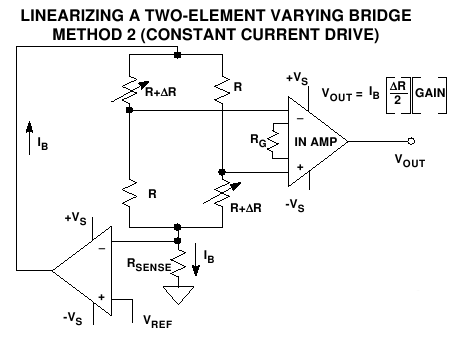
\includegraphics[width=15cm]{./img/circuit}
	\caption{Circuit conditionneur}
\end{figure}

La source de courant est bas�e sur l'amplificateur OPA335, avec en entr�e une r�f�rence de tension de 2,5~V (MCP1525). Tous les �l�ments apparaissant sur ce sch�ma doivent �tre au maximum ind�pendant de la temp�rature. Les r�sistances sont choisies avec une pr�cision d'au moins 0,1~\%.

Les r�sistances du pont de Wheatstone sont de 100,00~Ohm pour avoir un �quilibre � 0,00~�C. Il est compos� de deux �l�ments variants (des Pt100) pour avoir une erreur de lin�arit� nulle.\newline

La carte �mettrices est compos�e de quatres r�gulateurs. Le premier est un r�gulateur 5~V pour alimenter le PIC. Il est suivit d'un r�gulateur 3,3~V pour alimenter le module Xbee. Ce dernier r�gulateur dispose d'une broche de validation contr�l�e par le PIC. De cette mani�re, le PIC d�vide ou non d'aliment le module Xbee.

En parall�le est positionn� un r�gulateur 5~V d�di� � l'alimentation des amplificateurs unipolaires pour la mesure de temp�rature. Lui aussi dispose d'une entr�e de validation conn�ct� au PIC. Il est suivit de la r�f�rence de tension 2,5~V. En arr�tant ce r�gulateur 5~V, le PIC d�cide d'�teindre toute la cha�ne de mesure. \newline

De part cette alimentation, en quelques instants seulement il ne reste plus que le PIC d'aliment�. Celui-ci disposant d'une fonction \og veille \fg\  , lors d'une attente de mesure, la consommation est minime. De l'orde de quelque dizaines de micro-volts.\newline

Sur les diff�rentes cartes, beaucoup d'entr�es/sorties du module Xbee ont �t� connect�s. Ceci simplement pour une utilisation future. 

D'indispensable il n'y a pour l'instant que les broches suivantes~: DIN et DOUT pour la liaison s�rie et les commandes AT, contr�lant le module~; RTS et CTS pour contr�ler les tampons d'�mission et de r�ception~; SLEEP permettant de mettre en veille le module, associ�e � SLEEP\_RQ pour v�rifier l'�tat du module.

Le sch�ma ainsi que les typons sont disponibles en annexe.


%%
\subsection{Le module Xbee} \label{zigbee}
Le 

%%%%
\subsection{Le programme}
la source du prog.
Les am�liorations envisageables.
%%%



 \newpage
\section*{Conclusion}
\addcontentsline{toc}{section}{Conclusion}

qsfq sqf
 

\newpage
%% Annexes

\appendix

\section{table Pt100}

Table de r�sistivit� de la Pt100 (valeur � multiplier par 10 pour avoir la table de la Pt1000)


\large{Selon ITS-90/DIN EN 60751}
Unit�s : T en \degres C et R en $\Omega$


\vspace{4mm}
%\begin{table}
\footnotesize{
\begin{changemargin}{-15mm}{-10mm}
\begin{center}
\begin{supertabular}{|c||c|c|c|c|c|c|c|c|c|c||c|}

   	\hline
	\textbf{\degres C} & \textbf{0} & \textbf{1} & \textbf{2} & \textbf{3} & \textbf{4} & \textbf{5} & \textbf{6} & \textbf{7} & \textbf{8} & \textbf{9} & \textbf{\degres C}\\\hline\hline
	-200.00&  18.52& & & & & & & & & &                                              -200.00 \\\hline
	-190.00&  22.83&  22.40&  21.97&  21.54&  21.11&  20.68&  20.25&  19.82&  19.38&  18.95& -190.00 \\\hline
	-180.00&  27.10&  26.67&  26.24&  25.82&  25.39&  24.97&  24.54&  24.11&  23.68&  23.25& -180.00 \\\hline
	-170.00&  31.34&  30.91&  30.49&  30.07&  29.64&  29.22&  28.80&  28.37&  27.95&  27.52& -170.00 \\\hline
	-160.00&  35.54&  35.12&  34.70&  34.28&  33.86&  33.44&  33.02&  32.60&  32.18&  31.76& -160.00 \\\hline
	-150.00&  39.72&  39.31&  38.89&  38.47&  38.05&  37.64&  37.22&  36.80&  36.38&  35.96& -150.00 \\\hline
	-140.00&  43.88&  43.46&  43.05&  42.63&  42.22&  41.80&  41.39&  40.97&  40.56&  40.14& -140.00 \\\hline
	-130.00&  48.00&  47.59&  47.18&  46.77&  46.36&  45.94&  45.53&  45.12&  44.70&  44.29& -130.00 \\\hline
	-120.00&  52.11&  51.70&  51.29&  50.88&  50.47&  50.06&  49.65&  49.24&  48.83&  48.42& -120.00 \\\hline
	-110.00&  56.19&  55.79&  55.38&  54.97&  54.56&  54.15&  53.75&  53.34&  52.93&  52.52& -110.00 \\\hline
	-100.00&  60.26&  59.85&  59.44&  59.04&  58.63&  58.23&  57.82&  57.41&  57.01&  56.60& -100.00 \\\hline
	 -90.00&  64.30&  63.90&  63.49&  63.09&  62.68&  62.28&  61.88&  61.47&  61.07&  60.66&  -90.00 \\\hline
	 -80.00&  68.33&  67.92&  67.52&  67.12&  66.72&  66.31&  65.91&  65.51&  65.11&  64.70&  -80.00 \\\hline
	 -70.00&  72.33&  71.93&  71.53&  71.13&  70.73&  70.33&  69.93&  69.53&  69.13&  68.73&  -70.00 \\\hline
	 -60.00&  76.33&  75.93&  75.53&  75.13&  74.73&  74.33&  73.93&  73.53&  73.13&  72.73&  -60.00 \\\hline
	 -50.00&  80.31&  79.91&  79.51&  79.11&  78.72&  78.32&  77.92&  77.52&  77.12&  76.73&  -50.00 \\\hline
	 -40.00&  84.27&  83.87&  83.48&  83.08&  82.69&  82.29&  81.89&  81.50&  81.10&  80.70&  -40.00 \\\hline
	 -30.00&  88.22&  87.83&  87.43&  87.04&  86.64&  86.25&  85.85&  85.46&  85.06&  84.67&  -30.00 \\\hline
	 -20.00&  92.16&  91.77&  91.37&  90.98&  90.59&  90.19&  89.80&  89.40&  89.01&  88.62&  -20.00 \\\hline
	 -10.00&  96.09&  95.69&  95.30&  94.91&  94.52&  94.12&  93.73&  93.34&  92.95&  92.55&  -10.00 \\\hline
	   0.00& 100.00&  99.61&  99.22&  98.83&  98.44&  98.04&  97.65&  97.26&  96.87&  96.48&    0.00 \\\hline
\hline
	\textbf{\degres C} & \textbf{0} & \textbf{1} & \textbf{2} & \textbf{3} & \textbf{4} & \textbf{5} & \textbf{6} & \textbf{7} & \textbf{8} & \textbf{9} & \textbf{\degres C}\\\hline\hline
	   0.00& 100.00& 100.39& 100.78& 101.17& 101.56& 101.95& 102.34& 102.73& 103.12& 103.51&    0.00 \\\hline
	  10.00& 103.90& 104.29& 104.68& 105.07& 105.46& 105.85& 106.24& 106.63& 107.02& 107.40&   10.00 \\\hline
	  20.00& 107.79& 108.18& 108.57& 108.96& 109.35& 109.73& 110.12& 110.51& 110.90& 111.29&   20.00 \\\hline
	  30.00& 111.67& 112.06& 112.45& 112.83& 113.22& 113.61& 114.00& 114.38& 114.77& 115.15&   30.00 \\\hline
	  40.00& 115.54& 115.93& 116.31& 116.70& 117.08& 117.47& 117.86& 118.24& 118.63& 119.01&   40.00 \\\hline
	  50.00& 119.40& 119.78& 120.17& 120.55& 120.94& 121.32& 121.71& 122.09& 122.47& 122.86&   50.00 \\\hline
	  60.00& 123.24& 123.63& 124.01& 124.39& 124.78& 125.16& 125.54& 125.93& 126.31& 126.69&   60.00 \\\hline
	  70.00& 127.08& 127.46& 127.84& 128.22& 128.61& 128.99& 129.37& 129.75& 130.13& 130.52&   70.00 \\\hline
	  80.00& 130.90& 131.28& 131.66& 132.04& 132.42& 132.80& 133.18& 133.57& 133.95& 134.33&   80.00 \\\hline
	  90.00& 134.71& 135.09& 135.47& 135.85& 136.23& 136.61& 136.99& 137.37& 137.75& 138.13&   90.00 \\\hline
	 100.00& 138.51& 138.88& 139.26& 139.64& 140.02& 140.40& 140.78& 141.16& 141.54& 141.91&  100.00 \\\hline
	 110.00& 142.29& 142.67& 143.05& 143.43& 143.80& 144.18& 144.56& 144.94& 145.31& 145.69&  110.00 \\\hline
	 120.00& 146.07& 146.44& 146.82& 147.20& 147.57& 147.95& 148.33& 148.70& 149.08& 149.46&  120.00 \\\hline
	 130.00& 149.83& 150.21& 150.58& 150.96& 151.33& 151.71& 152.08& 152.46& 152.83& 153.21&  130.00 \\\hline
	 140.00& 153.58& 153.96& 154.33& 154.71& 155.08& 155.46& 155.83& 156.20& 156.58& 156.95&  140.00 \\\hline
	 150.00& 157.33& 157.70& 158.07& 158.45& 158.82& 159.19& 159.56& 159.94& 160.31& 160.68&  150.00 \\\hline
	 160.00& 161.05& 161.43& 161.80& 162.17& 162.54& 162.91& 163.29& 163.66& 164.03& 164.40&  160.00 \\\hline
	 170.00& 164.77& 165.14& 165.51& 165.89& 166.26& 166.63& 167.00& 167.37& 167.74& 168.11&  170.00 \\\hline 
	 180.00& 168.48& 168.85& 169.22& 169.59& 169.96& 170.33& 170.70& 171.07& 171.43& 171.80&  180.00 \\\hline
	 190.00& 172.17& 172.54& 172.91& 173.28& 173.65& 174.02& 174.38& 174.75& 175.12& 175.49&  190.00 \\\hline
\hline
	\textbf{\degres C} & \textbf{0} & \textbf{1} & \textbf{2} & \textbf{3} & \textbf{4} & \textbf{5} & \textbf{6} & \textbf{7} & \textbf{8} & \textbf{9} & \textbf{\degres C}\\\hline\hline
	 200.00& 175.86& 176.22& 176.59& 176.96& 177.33& 177.69& 178.06& 178.43& 178.79& 179.16&  200.00 \\\hline
	 210.00& 179.53& 179.89& 180.26& 180.63& 180.99& 181.36& 181.72& 182.09& 182.46& 182.82&  210.00 \\\hline
	 220.00& 183.19& 183.55& 183.92& 184.28& 184.65& 185.01& 185.38& 185.74& 186.11& 186.47&  220.00 \\\hline
	 230.00& 186.84& 187.20& 187.56& 187.93& 188.29& 188.66& 189.02& 189.38& 189.75& 190.11&  230.00 \\\hline
	 240.00& 190.47& 190.84& 191.20& 191.56& 191.92& 192.29& 192.65& 193.01& 193.37& 193.74&  240.00 \\\hline
	 250.00& 194.10& 194.46& 194.82& 195.18& 195.55& 195.91& 196.27& 196.63& 196.99& 197.35&  250.00 \\\hline
	 260.00& 197.71& 198.07& 198.43& 198.79& 199.15& 199.51& 199.87& 200.23& 200.59& 200.95&  260.00 \\\hline
	 270.00& 201.31& 201.67& 202.03& 202.39& 202.75& 203.11& 203.47& 203.83& 204.19& 204.55&  270.00 \\\hline
	 280.00& 204.90& 205.26& 205.62& 205.98& 206.34& 206.70& 207.05& 207.41& 207.77& 208.13&  280.00 \\\hline
	 290.00& 208.48& 208.84& 209.20& 209.56& 209.91& 210.27& 210.63& 210.98& 211.34& 211.70&  290.00 \\\hline
	 300.00& 212.05& 212.41& 212.76& 213.12& 213.48& 213.83& 214.19& 214.54& 214.90& 215.25&  300.00 \\\hline
	 310.00& 215.61& 215.96& 216.32& 216.67& 217.03& 217.38& 217.74& 218.09& 218.44& 218.80&  310.00 \\\hline
	 320.00& 219.15& 219.51& 219.86& 220.21& 220.57& 220.92& 221.27& 221.63& 221.98& 222.33&  320.00 \\\hline 
  	 330.00& 222.68& 223.04& 223.39& 223.74& 224.09& 224.45& 224.80& 225.15& 225.50& 225.85& 330.00 \\\hline
	 340.00& 226.21& 226.56& 226.91& 227.26& 227.61& 227.96& 228.31& 228.66& 229.02& 229.37& 340.00 \\\hline
	 350.00& 229.72& 230.07& 230.42& 230.77& 231.12& 231.47& 231.82& 232.17& 232.52& 232.87& 350.00 \\\hline
	 360.00& 233.21& 233.56& 233.91& 234.26& 234.61& 234.96& 235.31& 235.66& 236.00& 236.35& 360.00 \\\hline
	 370.00& 236.70& 237.05& 237.40& 237.74& 238.09& 238.44& 238.79& 239.13& 239.48& 239.83& 370.00 \\\hline
	 380.00& 240.18& 240.52& 240.87& 241.22& 241.56& 241.91& 242.26& 242.60& 242.95& 243.29& 380.00 \\\hline
	 390.00& 243.64& 243.99& 244.33& 244.68& 245.02& 245.37& 245.71& 246.06& 246.40& 246.75& 390.00 \\\hline
\hline
	\textbf{\degres C} & \textbf{0} & \textbf{1} & \textbf{2} & \textbf{3} & \textbf{4} & \textbf{5} & \textbf{6} & \textbf{7} & \textbf{8} & \textbf{9} & \textbf{\degres C}\\\hline\hline
	 400.00& 247.09& 247.44& 247.78& 248.13& 248.47& 248.81& 249.16& 249.50& 249.85& 250.19& 400.00 \\\hline
	 410.00& 250.53& 250.88& 251.22& 251.56& 251.91& 252.25& 252.59& 252.93& 253.28& 253.62& 410.00 \\\hline
	 420.00& 253.96& 254.30& 254.65& 254.99& 255.33& 255.67& 256.01& 256.35& 256.70& 257.04& 420.00 \\\hline
	 430.00& 257.38& 257.72& 258.06& 258.40& 258.74& 259.08& 259.42& 259.76& 260.10& 260.44& 430.00 \\\hline
	 440.00& 260.78& 261.12& 261.46& 261.80& 262.14& 262.48& 262.82& 263.16& 263.50& 263.84& 440.00 \\\hline
	 450.00& 264.18& 264.52& 264.86& 265.20& 265.53& 265.87& 266.21& 266.55& 266.89& 267.22& 450.00 \\\hline
	 460.00& 267.56& 267.90& 268.24& 268.57& 268.91& 269.25& 269.59& 269.92& 270.26& 270.60& 460.00 \\\hline
	 470.00& 270.93& 271.27& 271.61& 271.94& 272.28& 272.61& 272.95& 273.29& 273.62& 273.96& 470.00 \\\hline
	 480.00& 274.29& 274.63& 274.96& 275.30& 275.63& 275.97& 276.30& 276.64& 276.97& 277.31& 480.00 \\\hline
	 490.00& 277.64& 277.98& 278.31& 278.64& 278.98& 279.31& 279.64& 279.98& 280.31& 280.64& 490.00 \\\hline
	 500.00& 280.98& 281.31& 281.64& 281.98& 282.31& 282.64& 282.97& 283.31& 283.64& 283.97& 500.00 \\\hline
	 510.00& 284.30& 284.63& 284.97& 285.30& 285.63& 285.96& 286.29& 286.62& 286.95& 287.29& 510.00 \\\hline
	 520.00& 287.62& 287.95& 288.28& 288.61& 288.94& 289.27& 289.60& 289.93& 290.26& 290.59& 520.00 \\\hline
	 530.00& 290.92& 291.25& 291.58& 291.91& 292.24& 292.56& 292.89& 293.22& 293.55& 293.88& 530.00 \\\hline
	 540.00& 294.21& 294.54& 294.86& 295.19& 295.52& 295.85& 296.18& 296.50& 296.83& 297.16& 540.00 \\\hline
	 550.00& 297.49& 297.81& 298.14& 298.47& 298.80& 299.12& 299.45& 299.78& 300.10& 300.43& 550.00 \\\hline
	 560.00& 300.75& 301.08& 301.41& 301.73& 302.06& 302.38& 302.71& 303.03& 303.36& 303.69& 560.00 \\\hline
	 570.00& 304.01& 304.34& 304.66& 304.98& 305.31& 305.63& 305.96& 306.28& 306.61& 306.93& 570.00 \\\hline
	 580.00& 307.25& 307.58& 307.90& 308.23& 308.55& 308.87& 309.20& 309.52& 309.84& 310.16& 580.00 \\\hline
	 590.00& 310.49& 310.81& 311.13& 311.45& 311.78& 312.10& 312.42& 312.74& 313.06& 313.39& 590.00 \\\hline
\hline
	\textbf{\degres C} & \textbf{0} & \textbf{1} & \textbf{2} & \textbf{3} & \textbf{4} & \textbf{5} & \textbf{6} & \textbf{7} & \textbf{8} & \textbf{9} & \textbf{\degres C}\\\hline\hline
	 600.00& 313.71& 314.03& 314.35& 314.67& 314.99& 315.31& 315.64& 315.96& 316.28& 316.60& 600.00 \\\hline
	 610.00& 316.92& 317.24& 317.56& 317.88& 318.20& 318.52& 318.84& 319.16& 319.48& 319.80& 610.00 \\\hline
	 620.00& 320.12& 320.43& 320.75& 321.07& 321.39& 321.71& 322.03& 322.35& 322.67& 322.98& 620.00 \\\hline
	 630.00& 323.30& 323.62& 323.94& 324.26& 324.57& 324.89& 325.21& 325.53& 325.84& 326.16& 630.00 \\\hline
	 640.00& 326.48& 326.79& 327.11& 327.43& 327.74& 328.06& 328.38& 328.69& 329.01& 329.32& 640.00 \\\hline
	 650.00& 329.64& 329.96& 330.27& 330.59& 330.90& 331.22& 331.53& 331.85& 332.16& 332.48& 650.00 \\\hline
	 660.00& 332.79& 333.11& 333.42& 333.74& 334.05& 334.36& 334.68& 334.99& 335.31& 335.62& 660.00 \\\hline
	 670.00& 335.93& 336.25& 336.56& 336.87& 337.18& 337.50& 337.81& 338.12& 338.44& 338.75& 670.00 \\\hline
	 680.00& 339.06& 339.37& 339.69& 340.00& 340.31& 340.62& 340.93& 341.24& 341.56& 341.87& 680.00 \\\hline
	 690.00& 342.18& 342.49& 342.80& 343.11& 343.42& 343.73& 344.04& 344.35& 344.66& 344.97& 690.00 \\\hline
	 700.00& 345.28& 345.59& 345.90& 346.21& 346.52& 346.83& 347.14& 347.45& 347.76& 348.07& 700.00 \\\hline
	 710.00& 348.38& 348.69& 348.99& 349.30& 349.61& 349.92& 350.23& 350.54& 350.84& 351.15& 710.00 \\\hline
	 720.00& 351.46& 351.77& 352.08& 352.38& 352.69& 353.00& 353.30& 353.61& 353.92& 354.22& 720.00 \\\hline
	 730.00& 354.53& 354.84& 355.14& 355.45& 355.76& 356.06& 356.37& 356.67& 356.98& 357.28& 730.00 \\\hline
	 740.00& 357.59& 357.90& 358.20& 358.51& 358.81& 359.12& 359.42& 359.72& 360.03& 360.33& 740.00 \\\hline
	 750.00& 360.64& 360.94& 361.25& 361.55& 361.85& 362.16& 362.46& 362.76& 363.07& 363.37& 750.00 \\\hline
	 760.00& 363.67& 363.98& 364.28& 364.58& 364.89& 365.19& 365.49& 365.79& 366.10& 366.40& 760.00 \\\hline
	 770.00& 366.70& 367.00& 367.30& 367.60& 367.91& 368.21& 368.51& 368.81& 369.11& 369.41& 770.00 \\\hline
	 780.00& 369.71& 370.01& 370.31& 370.61& 370.91& 371.21& 371.51& 371.81& 372.11& 372.41& 780.00 \\\hline
	 790.00& 372.71& 373.01& 373.31& 373.61& 373.91& 374.21& 374.51& 374.81& 375.11& 375.41& 790.00 \\\hline
	 800.00& 375.70& 376.00& 376.30& 376.60& 376.90& 377.19& 377.49& 377.79& 378.09& 378.39& 800.00 \\\hline
	 810.00& 378.68& 378.98& 379.28& 379.57& 379.87& 380.17& 380.46& 380.76& 381.06& 381.35& 810.00 \\\hline
	 820.00& 381.65& 381.95& 382.24& 382.54& 382.83& 383.13& 383.42& 383.72& 384.01& 384.31& 820.00 \\\hline
	 830.00& 384.60& 384.90& 385.19& 385.49& 385.78& 386.08& 386.37& 386.67& 386.96& 387.25& 830.00 \\\hline
	 840.00& 387.55& 387.84& 388.14& 388.43& 388.72& 389.02& 389.31& 389.60& 389.90& 390.19& 840.00 \\\hline
	 850.00& 390.48&       &       &       &       &       &       &       &       &       & 850.00 \\\hline
\hline
	\textbf{\degres C} & \textbf{0} & \textbf{1} & \textbf{2} & \textbf{3} & \textbf{4} & \textbf{5} & \textbf{6} & \textbf{7} & \textbf{8} & \textbf{9} & \textbf{\degres C}\\\hline\hline

\end{supertabular}
\end{center}
\caption{Table Pt100}
\end{changemargin}
}

%\end{table}


\thispagestyle{empty}

\chapter{Calcul d'incertitude} \label{Incertitude}
%%%
\normalsize
Ici nous allons effectuer en d�tail les calculs d'incertitude pour estimer la pr�cision de la cha�ne de mesure.
Ceci dans le but de conna�tre l'incertitudes des mesures de temp�ratures envoy�es par le PIC. Les calculs seraient all�g�s en utilisant les d�riv�es logarithmiques, mais j'ai pr�f�r� n'utiliser qu'une seule m�thode.


\section{Donn�es}
Les documentations constructeurs nous donnent~:\newline
$R_s=1~k\Omega\ � 0,1\%$;\newline
$R=100~\Omega\ � 0,1\%$;\newline
$R_{Pt100}=(R_0+\delta R)~\Omega\ $ � $0,01\%$. Pour la suite on choisira $R_0=R$ pour avoir $R_0$ � $0,1\%$ et $\delta R $ � $0,01\%$;\newline
Pour une temp�rature sup�rieure � $\theta =0~\tccentigrade$, on � $2,498~V\leq V_{ref}\leq 2,500~V$. \newline
L'OPA335 a++++ un offset d'entr�e de $5~\mu V$ et l'amplificateur d'instrumentation (INA118) un offset de $50~\mu V$;\newline
$R_g$ la r�sistance de gain, est � 0,1\%. \newline

Soit $T$ la temp�rature et $T_0$ la temp�rature de r�f�rence (0,00~\degres C dans notre cas). Pour les calculs d'incertitudes pour le cas le plus d�favorable, on choisit la temp�rature la plus �loign�e, $\theta = 30~\tccentigrade$.

\section{Les �tapes}
\subsection*{Incertitude absolue de $V_{ref}$}
$V_{ref}=\overline{V_{ref}}\pm \Delta V_{ref}$\newline
\begin{equation}
\fbox{$V_{ref}=(2,499\pm 0,001)~V$}
\end{equation}
\subsection*{Incertitude absolue sur $R_s$, $R$ et $\delta R$}
$\Delta R_s=(R_s\times 0,1\%)~\Omega$. Soit~:
\begin{equation}
\fbox{$R_s=(1000\pm 1)~\Omega$}\newline
\end{equation}
De m�me on trouve 
\begin{equation}
\fbox{$R=(100\pm 0,1)~\Omega$}\newline
\end{equation}
Pour calculer l'incertitude sur $\delta R$ on choisira le cas le plus d�favorable, c'est-�-dire la plus grande variation � mesurer. Pour $\delta R(\theta)=11,67~\Omega$. 

D'o� $\Delta \delta R=(\delta R(\theta)\times 0,01\%)=0,0012~\Omega$. Finalement, 
\begin{equation}
\fbox{$\delta R=(\delta R\pm 0,001)~\Omega$}
\end{equation}

\subsection*{Incertitude absolue sur $I$}
On a $I=\frac{V_{ref}}{R_s}$\newline
$$dI=\frac{\partial I}{\partial V_{ref}}dV_{ref} + \frac{\partial I}{\partial R_s}dR_s=\frac{1}{R_s}dV_{ref}-\frac{V_{ref}}{R_s^2}dR_s$$ \newline
On en d�duit l'incertitude relative $\Delta I$~:

$$\Delta I=\left|\frac{1}{R_s}\right|\Delta V_{ref}+\left|\frac{-V_{ref}}{R_s^2}\right|\Delta R_s$$ \newline
Application num�rique~:$\Delta I=\left|\frac{1}{100}\right|\times 0,001+\left|\frac{-2,499}{100^2}\right|\times 1$. D'o�~:
\begin{equation}
\fbox{$I=(2,499\pm 0,004)~mA$}
\end{equation}
\subsection*{Incertitude absolue sur $V_0$}
Soient $V_A$ et $V_B$ tels que $V_0=V_A-V_B$ et $I'$ le courant traversant une sonde. Il faut avant tout d�terminer $\Delta I'$.

\subsubsection{Incertitude sur $I'$}
$I'=I\frac{2R+\delta R}{4R+2\delta R}=\frac{I}{2}=1,2495$. D'o� la diff�rentielle suivante~: 
\begin{eqnarray*}
dI'&=&\frac{\partial I'}{\partial I}dI \\
\Delta I'& = & \left|\frac{1}{2}\right|\Delta I=1,7\mu A
\end{eqnarray*}

\begin{equation}
\fbox{$I'=(1,250\pm 0,002)~mA$}
\end{equation}

\subsubsection{Incertitude sur $V_A$}
On a $V_A=I'\times R$

\begin{eqnarray*}
dV_A & = &\frac{\partial V_A}{\partial I'}dI' + \frac{\partial V_A}{\partial R}dR \\
& = & RdI'+I'dR\\
\Delta V_A & = & |R|\Delta I'+|I'|\Delta R
\end{eqnarray*}

\begin{equation}
\fbox{$\Delta V_A=0,325~mV$}
\end{equation}

\subsubsection{Incertitude sur $V_B$}
On a
$$V_B = I\frac{2R+\delta R}{4R+2\delta R}(2R+\delta R)=I\frac{(2R+\delta R)^2}{4R+2\delta R}$$

\begin{eqnarray*}
dV_B & = &\frac{\partial V_B}{\partial I}dI + \frac{\partial V_B}{\partial R}dR + \frac{\partial V_B}{\partial \delta R}d\delta R\\
& = &\frac{(2R+\delta R)^2}{4R+2\delta R}dI +I\frac{(8R+4\delta R)(4R+2\delta R)-4(2R+\delta R)^2}{(4R+2\delta R)^2}dR +\\
& &  I\frac{(4R+2\delta R)(4R+2\delta R)-2(2R+\delta R)^2}{(4R+2\delta R)^2}d\delta R\\
& = & \frac{(2R+\delta R)^2}{4R+2\delta R}dI +I\frac{16R^2-8\delta R^2}{(4R+2\delta R)^2}dR + I\frac{1}{2}d\delta R
\end{eqnarray*}
Pour un cas g�n�ral on obtient donc~:
\begin{equation}
\fbox{$\Delta V_B=\left|\frac{(2R+\delta R)^2}{4R +\delta R}\right|\Delta I+\left|I\frac{16R^2-8\delta R^2}{(4R+2\delta R)^2}\right|\Delta R+\left|\frac{1}{2}\right|\Delta \delta R$}
\end{equation}

Dans notre �tude, nous allons prendre le cas le plus d�favorable, c'est-�-dire $T=\theta$. Soit $\delta R=11,67~\Omega$.\newline
Application num�rique~:
\begin{equation}
\fbox{$\Delta V_B(\delta R(\theta))=1,157~mV$}
\end{equation}

\subsubsection{Incertitude sur $V_0$}
En reprenant le calcul r�alis� dans le rapport (page \pageref{V0}) on a~:$$V_0=\frac{I}{2}\times \delta R$$
Et pour l'incertitude, 
$$\Delta V_0=\Delta V_A+\Delta V_B=1,482~mV$$
D'o�
\begin{equation}
\fbox{$ V_0=(\frac{I}{2}\times \delta R\pm 1,482\times 10^{-3})~V$}
\end{equation}


\subsection*{Incertitude absolue sur $V_s$}
\subsubsection{Gain}
Soit $V_s$ le signal disponible en sortie de l'amplificateur d'instrumentation, et $R_g$ sa r�sistance de gain � 0,1\%. La d�termination de $R_g$ est issue de la formule disponible dans la documentation constructeur (voir ci-dessous) pour une pleine �chelle (0~V--5~V). 
\begin{equation}
\fbox{$R_g=(150\pm 0,15)~\Omega$}\newline
\end{equation}

On a 
\begin{eqnarray*}
G & = & 1+\frac{50\times 10^3~[\Omega]}{R_g}=334,33\\
dG & = & \frac{\partial G}{\partial R_g}dR_g = \frac{-200\times 10^3}{R_g^2}dR_g\\
\Delta G & = &  \left|\frac{50\times 10^3}{R_g^2}\right|\Delta R_g= 0,3333~\Omega 
\end{eqnarray*}

Soit
\begin{equation}
\fbox{$G=334,33\pm 0,3333$}\newline
\end{equation}

\subsubsection{Calcul de l'incertitude sur $V_s$}
\begin{eqnarray*}
V_s & = & V_0\times G\\
dV_s & = & \frac{\partial V_s}{\partial V_0}dV_0 + \frac{\partial V_s}{\partial G}dG=GdV_0+V_0dG\\
\Delta V_s(\theta) & = & G\cdot\Delta V_0 + V_0\cdot\Delta G
\end{eqnarray*}

Application num�rique pour $T=\theta$~:$\Delta V_s=0,5003~V$. On en d�duit donc que les $5~\mu$V d'offset de l'INA118 sont n�gligeables.

\begin{equation}
\fbox{$ V_s=(G\cdot\frac{I}{2}\cdot\delta R\pm 0,5003)~V$}
\end{equation}

\subsection*{Calcul final}
Des calculs pr�c�dents, on trouve (avec l'incertitude valable pour une plage 0--30~\degres C)~:
\begin{equation}
V_s=\left (G\cdot\frac{I}{2}\cdot\delta R \pm 0,5003\right )~V
\label{Vs}
\end{equation}

Les tables (annexe~\ref{tablePt100}) donnent la r�sistance standard $R_{Pt100}$ de la Pt100 � la temp�rature $T$, pour une r�sistance nominale $R_0=100,00$ Ohm � la temp�rature de r�f�rence $T_0=0~\tccentigrade $. D�pendance pouvant �tre approxim�e par la relation~:

$R_{Pt100}=R_0\left (1+A\cdot\Delta T +B\cdot\Delta T ^2\right )$, o�~: $\Delta T =T -T _0$. Avec $A=3,9083\times 10^{-3}~K^{-1}$ et $B=-5,775\times 10^{-7}~K^{-2}$.
Ce qui donne pour d�terminer la temp�rature~:
$T=T_0+\frac{\sqrt{A^2+4B\cdot r}-A}{2B}$, o� 
\begin{equation}
r=\frac{R_{Pt100}}{R_0}-1
\label{r}
\end{equation}


Or on a $R_0=R$ et $R_{Pt100}=R+\delta R$. Notre variable �tant $V_s$, la tension disponible en entr�e du PIC, il ne faut obtenir que $V_s$ pour calculer la temp�rature. On l'obtient par la relation \eqref{Vs}. Soit,
$$ \delta R=\frac{2V_s}{G\cdot I}$$

d'o�~:
	
 

\begin{eqnarray*}
r & = & \frac{R+ \delta R}{R}-1 = \frac{\delta R}{R} = \frac{2V_s}{G\cdot I\cdot R}\\
dr & = & \frac{\partial r}{\partial V_s}dV_s + \frac{\partial r}{\partial G}dG+ \frac{\partial r}{\partial I}dI+ \frac{\partial r}{\partial R}dR\\
& = & \frac{2}{G\cdot I\cdot R}dV_s-2V_s\left ( \frac{dG}{G^2\cdot I\cdot R} + \frac{dI}{G\cdot I^2\cdot R} + \frac{dR}{G\cdot I\cdot R^2} \right )\\
& = & \frac{2}{G\cdot I\cdot R}dV_s-2\frac{G\cdot I\cdot\delta R}{2}\left ( \frac{dG}{G^2\cdot I\cdot R} + \frac{dI}{G\cdot I^2\cdot R} + \frac{dR}{G\cdot I\cdot R^2} \right )\\
\Delta r & = & \frac{2}{G\cdot I\cdot R}\Delta V_s+\delta R\left ( \frac{\Delta G}{G\cdot R} + \frac{\Delta I}{I\cdot R} + \frac{\Delta R}{R^2} \right )
\end{eqnarray*}

Soit l'application num�rique pour le cas le plus d�favorable~: $\Delta r = 0,0124$


Finalement on obtient~:
\begin{equation}
\fbox{$T=T_0+\frac{\sqrt{A^2+4B\cdot r}-A}{2B}$}
\label{Tfin}
\end{equation}
Avec
\begin{equation}
\fbox{$r=\frac{2V_s}{G\cdot I\cdot R}\pm 0,0124 $}
\label{Rfin}
\end{equation}


\subsection*{Incertitude finale}
On reprend $r  =  \frac{\delta R(\theta)}{R}$ pour calculer l'incertitude sur $T$~:
\begin{eqnarray*}
T & = & T_0+\frac{\sqrt{A^2+4B\cdot r}-A}{2B}\\
dT & = & \frac{\partial T}{\partial r}dr = \frac{1}{2B}\cdot\frac{4B}{2\sqrt{A^2+4B\cdot r}}dr = \frac{1}{\sqrt{A^2+4B\cdot r}}dr\\
\Delta T & = & \left |\frac{1}{\sqrt{A^2+4B\cdot r}}\right | \Delta r
\end{eqnarray*}


Application num�rique~:$\Delta T = 0,066~\tccentigrade$


\subsection*{R�sultat}

Th�oriquement, on obtient une mesure fid�le � 0,1~\degres C (avec une marge de 0,03~\degres C). Avec pour relations~:
\begin{center}
	\shadowbox{
\vspace{4mm}
		\begin{Beqnarray} 
		T & = & \left (T_0+\frac{\sqrt{A^2+4B\cdot r}-A}{2B}\pm 0,07\right ) \tccentigrade \label{rslt}\\
		r & = & \frac{2V_s}{G\cdot I\cdot R}\pm 0,0124 \label{rslt2}\\
		A & = & 3,9083\cdot 10^{-3}~K^{-1} \\
		B & = & -5,775\cdot 10^{-7}~K^{-2}\\
		T_0 & = & 0,00~\tccentigrade
		\end{Beqnarray}
\vspace{4mm}
	}
\end{center}

Avec pour le circuit pr�sent�~:
\begin{eqnarray}
	G & = & 425,53\pm 0,4255 \\
	I & = & (2,499\pm 0,004)~mA \\
	R & = & (100\pm 0,1)~\Omega 
\end{eqnarray}



\end{document}


%%
